\documentclass{standalone}
\usepackage{tikz}
\usetikzlibrary[arrows,positioning,matrix]

\begin{document}
\begin{tikzpicture}
  \node[draw=none] (schematic) {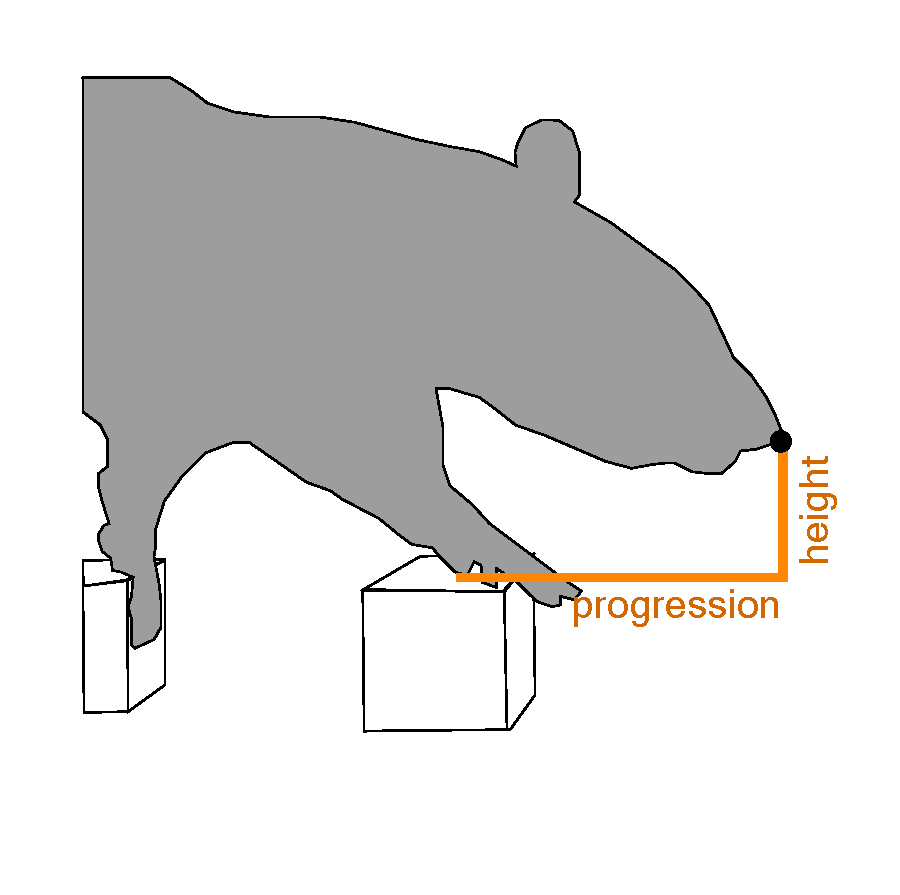
\includegraphics[width=0.33\textwidth]{elements/postureschematic}};
  \node[draw=none,above left=-5mm and -5mm of schematic] {A};

  \node[draw=none,right=1mm of schematic] (postureexample) {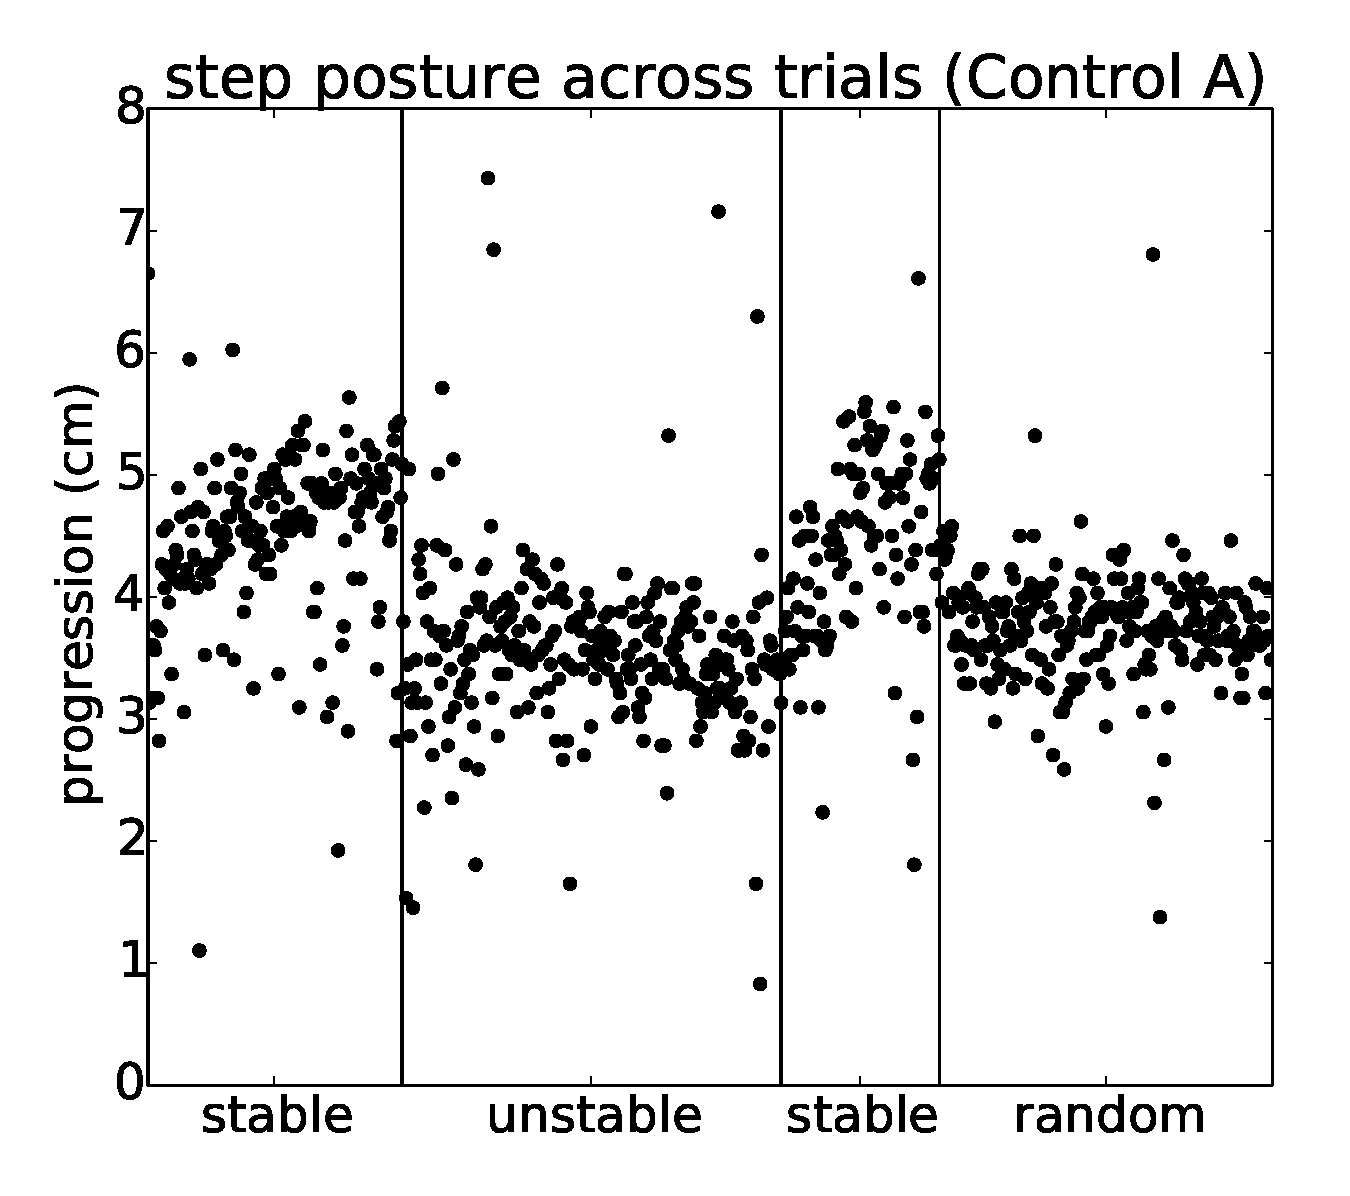
\includegraphics[width=0.33\textwidth]{elements/continuousposture}};
  \node[draw=none,above right=-5mm and 2mm of schematic] {B};
  
  \node[draw=none,right=1mm of postureexample] (posturesessions) {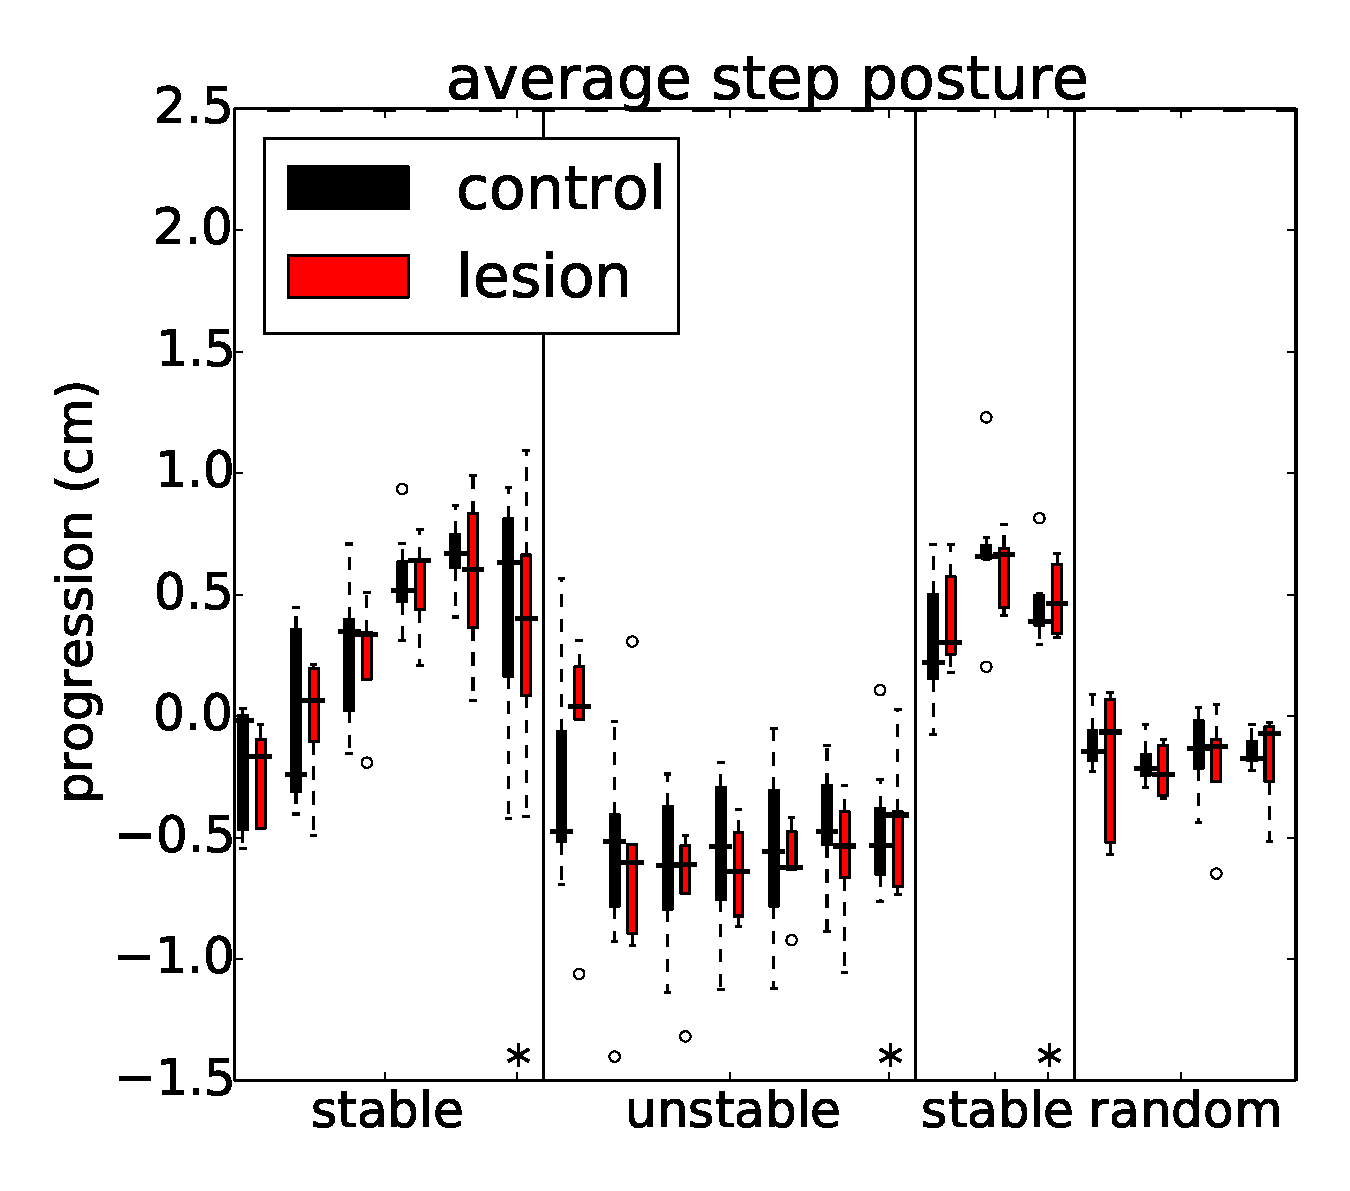
\includegraphics[width=0.33\textwidth]{elements/posturesessions}};
  \node[draw=none,above right=-5mm and 4.5cm of schematic] {C};

  \node[draw=none,below=0mm of schematic] (posturespeed) {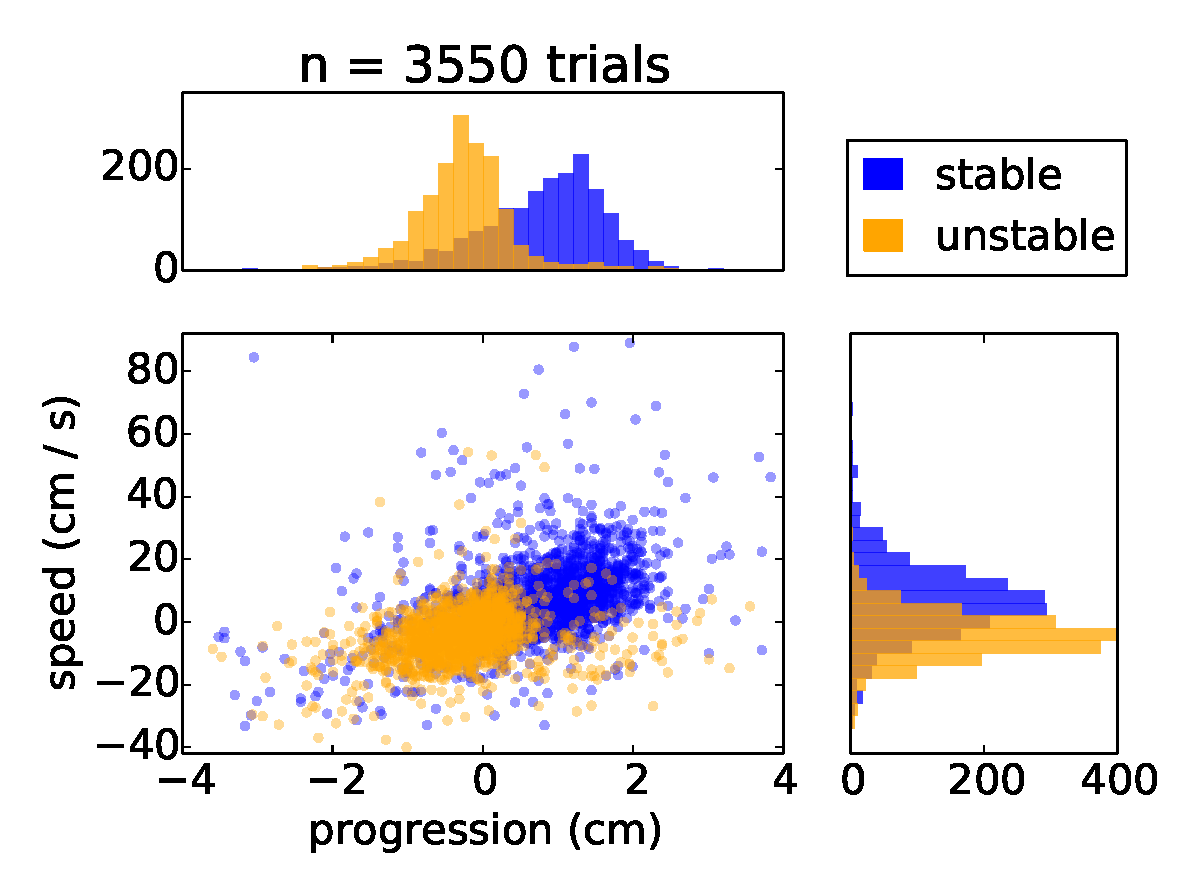
\includegraphics[width=0.33\textwidth]{elements/speedhistograms_b}};
  \node[draw=none,above=-2mm of posturespeed] {};
  \node[draw=none,above left=-2.5mm and -5mm of posturespeed] {D};
  
  \node[draw=none,right=1mm of posturespeed] (posturesmalllesions) {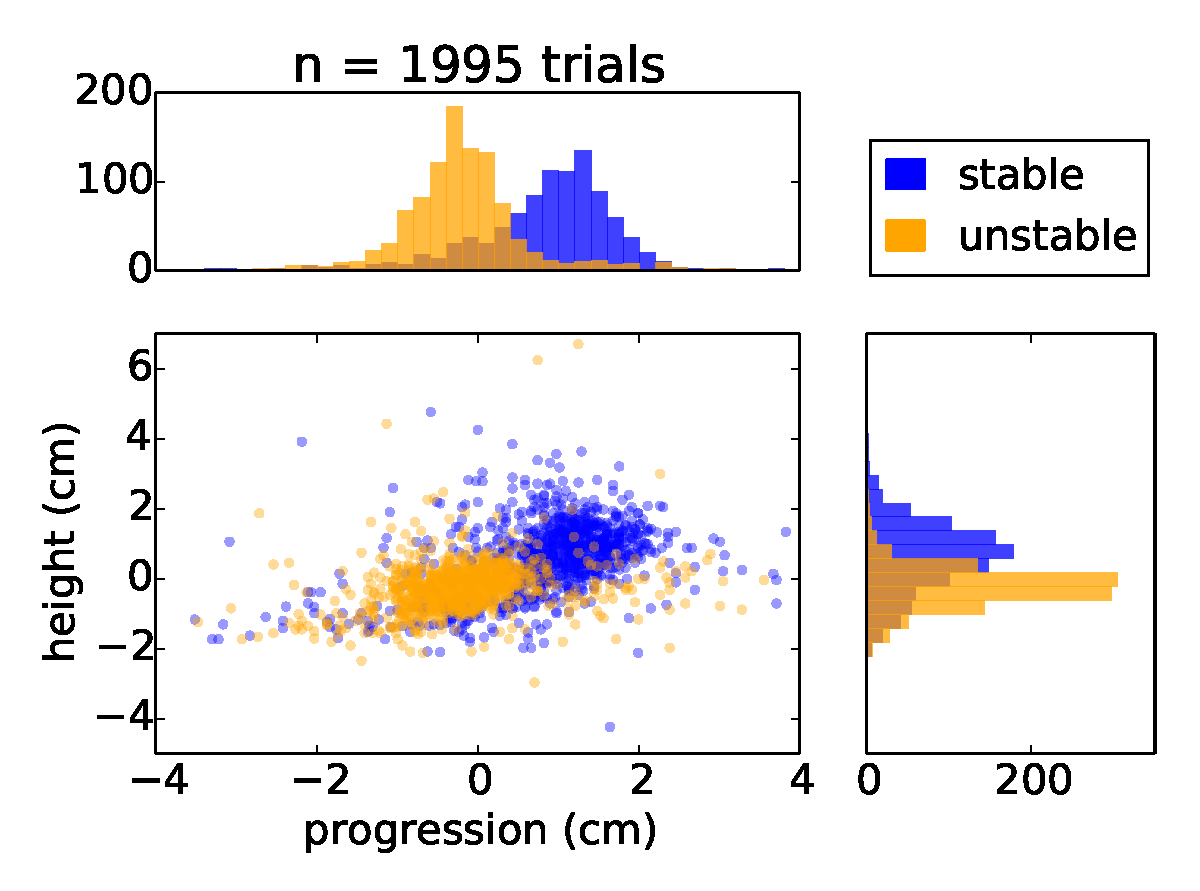
\includegraphics[width=0.33\textwidth]{elements/posturehistograms_controls_c}};
  \node[draw=none,above=-2mm of posturesmalllesions] {controls};
  \node[draw=none,above left=-2.5mm and -6mm of posturesmalllesions] {E};
  
  \node[draw=none,right=1mm of posturesmalllesions] (posturelesions) {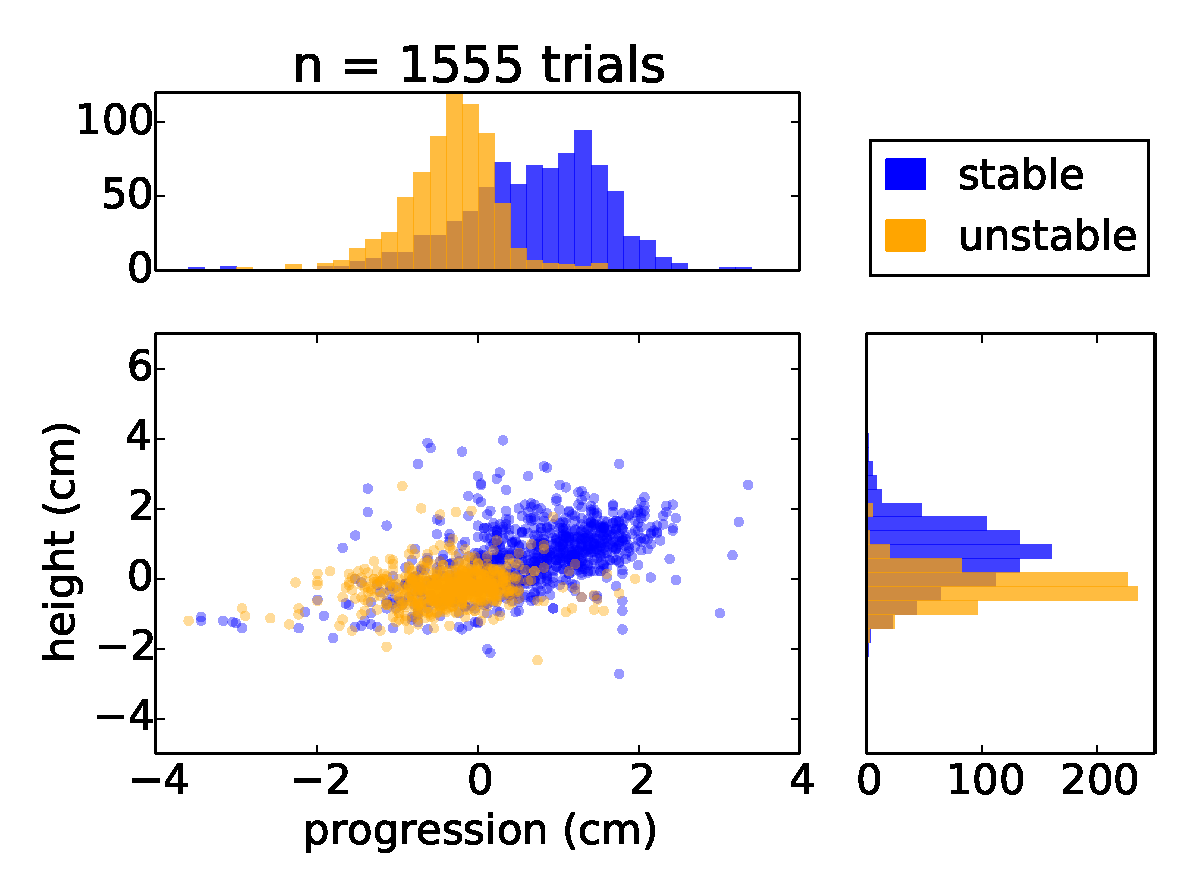
\includegraphics[width=0.33\textwidth]{elements/posturehistograms_alllesions_c}};
  \node[draw=none,above=-2.5mm of posturelesions] {lesions};
  \node[draw=none,above left=-2.5mm and -6mm of posturelesions] {F};
\end{tikzpicture}
\end{document}